\section{When Is Retrieving Raw Memory Enough?}
\label{sec:prelim}

To locate where the simple baseline stops being sufficient, we compare cosine retrieval of raw memory with full-context reading under a fixed reader, prompt, and judge. All runs in this section use \texttt{gemini-3.8-flash} as the reader and \texttt{gemini-embedding-2} as the retriever; Section~\ref{sec:setup} describes the shared protocol, and differences are paired over the same questions with 95\% bootstrap intervals.

\begin{table}[t]
\centering
\caption{Raw retrieval versus full-context reading with the same reader (\texttt{gemini-3.8-flash}). $\Delta$ is the paired difference from full context with a 95\% bootstrap interval; tokens are prompt tokens per question. LoCoMo and LongMemEval-S use the strict LongMemEval judge; MemEye uses its official 0--1 rubric. ``Annotated evidence'' reads only the gold evidence turns or rounds.}
\label{tab:prelim}
\small
\resizebox{\linewidth}{!}{%
\begin{tabular}{llccr}
\toprule
Benchmark & Condition & Accuracy & $\Delta$ vs.\ full context & Tokens \\
\midrule
\multirow{4}{*}{LoCoMo (1,540 q)} & Full context & 0.790 & -- & 32,499 \\
 & Cosine top-100 turns & 0.781 & $-0.009$ $[-0.023, +0.006]$ & 5,693 \\
 & Cosine top-10 turns & 0.706 & $-0.084$ $[-0.105, -0.064]$ & 755 \\
 & Annotated evidence & 0.739 & $-0.051$ $[-0.071, -0.031]$ & 435 \\
\midrule
\multirow{3}{*}{LongMemEval-S (119 q)} & Full context & 0.950 & -- & 113,227 \\
 & Cosine top-50 rounds & 0.941 & $-0.008$ $[-0.034, +0.017]$ & 21,730 \\
 & Cosine top-10 rounds & 0.899 & $-0.050$ $[-0.092, -0.017]$ & 4,986 \\
\midrule
\multirow{7}{*}{MemEye (371 q)} & Full context, images at low resolution & 0.819 & -- & 27,232 \\
 & Full context, images at high resolution & 0.811 & $-0.008$ $[-0.036, +0.020]$ & 78,961 \\
 & Full context, dense captions instead of images & 0.779 & $-0.040$ $[-0.077, -0.005]$ & 55,309 \\
 & Full context, no visual information & 0.191 & -- & 11,262 \\
 & Cosine top-40 rounds, images & 0.741 & $-0.079$ $[-0.112, -0.047]$ & 11,136 \\
 & Cosine top-10 rounds, images & 0.689 & $-0.130$ $[-0.173, -0.090]$ & 3,916 \\
 & Annotated evidence, images & 0.746 & $-0.073$ $[-0.115, -0.034]$ & 2,039 \\
\bottomrule
\end{tabular}}
\end{table}

\paragraph{Text memory.} Table~\ref{tab:prelim} reports LoCoMo~\citep{maharana2024locomo} (1,540 questions) and a stratified subset of LongMemEval-S~\citep{wu2025longmemeval} (119 questions). With a large budget, cosine retrieval is within one point of full-context reading on both benchmarks, and the intervals of the paired differences include zero. The gap opens only at small budgets, for example $-0.084$ for top-10 retrieval on LoCoMo. Reading only the annotated evidence turns of LoCoMo is 0.051 below full context, which suggests that annotated evidence often omits context that the answer needs. These results confirm the reported observation and qualify it: raw retrieval suffices on these benchmarks once its budget is large enough to contain the whole evidence.

\paragraph{Multimodal memory.} MemEye~\citep{guo2026memeye} contains 371 questions over eight life scenarios whose visual necessity was validated by its authors; removing all visual information leaves 0.191. Three observations distinguish it from text memory. First, reading the full history with every image at low resolution (about 266 tokens per image) reaches 0.819, which is 0.079 above top-40 retrieval; high resolution adds tokens but not accuracy. Second, replacing images by dense captions written at ingestion lowers accuracy to 0.779 and doubles the tokens, since a dense caption costs about 800 tokens, three times a low-resolution image. Third, captions are nevertheless useful as retrieval keys: the fraction of gold evidence rounds in the top 10 is 0.774 for a text-plus-caption key, 0.671 for a single embedding of text and image, and 0.300 for an image-only key (Appendix Table~\ref{tab:keys}), because relevant images score below unrelated text in the shared embedding space~\citep{liang2022modalitygap}. All later experiments therefore index rounds with captions but give readers the original images. The advantage of full context also depends on the reader: with a lighter reader, reading only the annotated evidence beats full context (Appendix Table~\ref{tab:reader}), so focused evidence matters more for weaker readers.

\paragraph{The residual gap is a set problem.} To find which questions retrieval loses, we split the gap between full context and top-10 retrieval by the number of gold evidence rounds. The gap is 0.038 for single-round questions ($n{=}119$), 0.125 for two or three rounds ($n{=}166$), and 0.267 for four or more ($n{=}86$); it is 0.034 when the retrieved rounds contain the complete evidence set ($n{=}235$) and 0.296 when they do not ($n{=}136$). Figure~\ref{fig:setsize} explains why larger budgets only postpone the problem: the probability that top-10 retrieval contains every gold round falls from 0.92 for single-round questions to 0.61, 0.32, and 0.00 as the set grows, and even top-40 retrieval recovers only 0.30 of sets with six or more rounds. Inspecting the misses shows that set members are often named by aliases defined elsewhere in the history: ``the D9 summary card'' is the summary shared in the ninth session, and ``the provisional busy-day trend'' is a screen from the session that opened with ``Busy day. I thought this snack might fit, but I'm not fully sure.'' None of these words occur in the round itself or in its caption.

\begin{figure}[t]
\centering
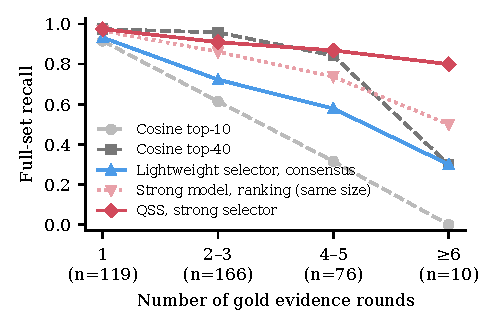
\includegraphics[width=0.48\linewidth]{figures/setsize.pdf}
\caption{Full-set recall on MemEye by the number of gold evidence rounds (371 questions; group sizes in parentheses). Dashed lines: cosine top-10 and top-40. \qss{} uses \texttt{gemini-3.8-flash} on a cosine prefilter of 100 candidates and opens 7.7 rounds on average; the ranking control lets the same model rank the same candidates and keeps, for every question, as many rounds as \qss{} selected. The lightweight selector applies sampling consensus with \texttt{gemini-2.5-flash-lite} (Section~\ref{sec:method}).}
\label{fig:setsize}
\end{figure}

These observations define four requirements. A memory retriever should be judged by whether it returns the complete evidence set (full-set recall), should spend a budget that grows with the size of the set, should resolve references against the structure of the history, and should leave the original images to the reader.
